\begin{multicols}{3}
\byline{Интервю}{СИЛВИЯ ДОБРЕВА 11Д}

\noindent \begin{window}[2,r, 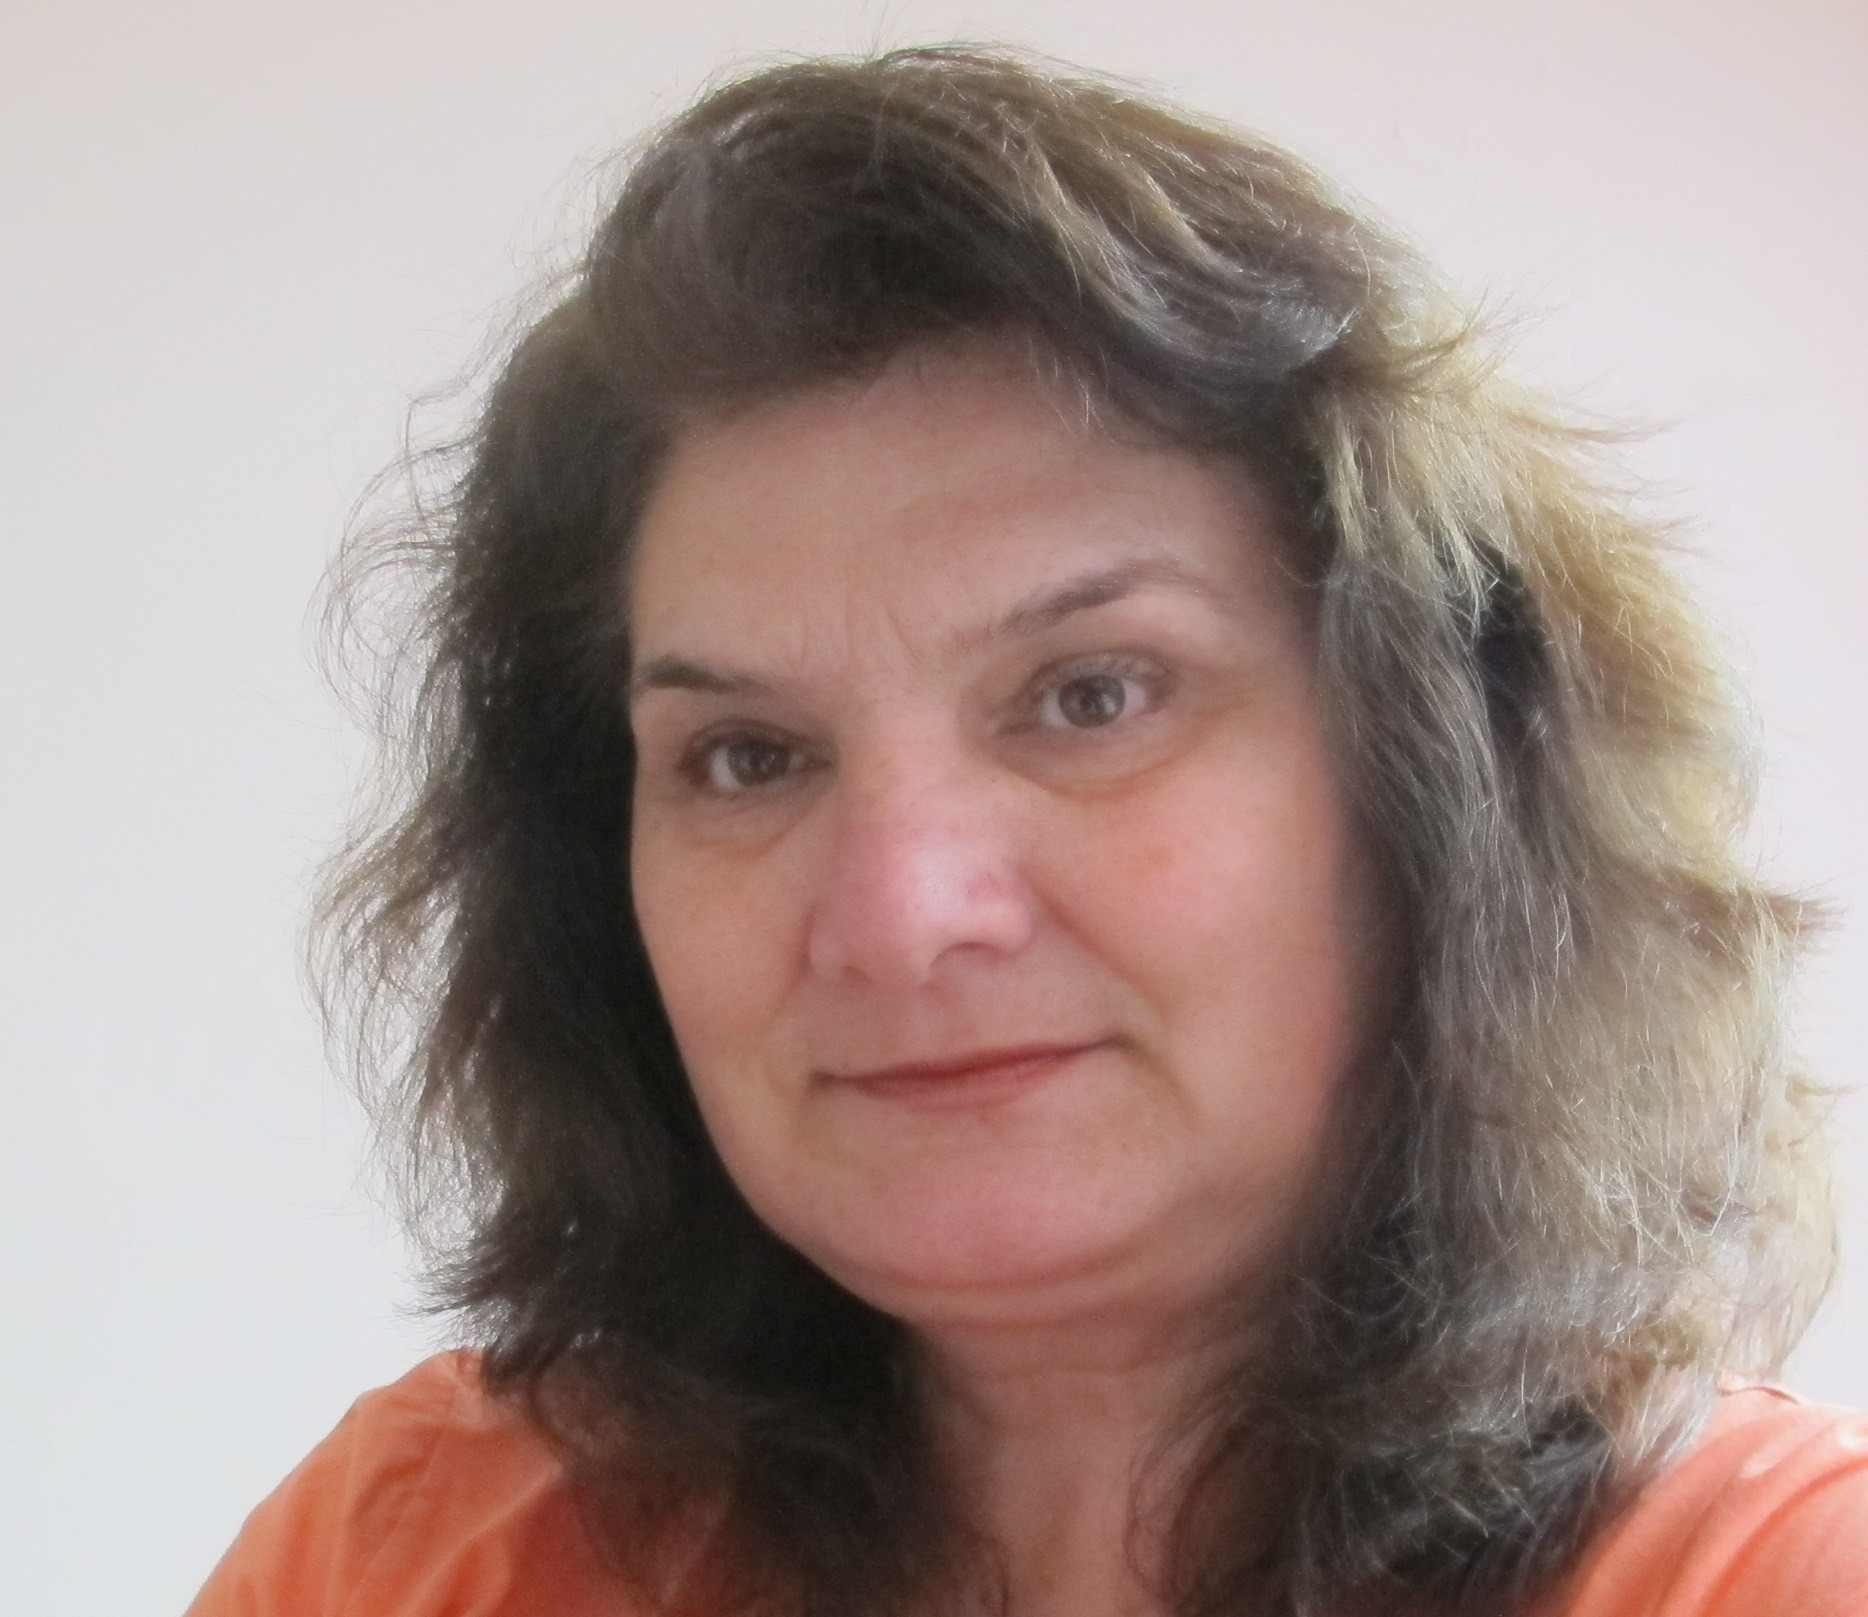
\includegraphics[width=2.1in]{./Radeva/IMG_3591.JPG},] \end{window}

Здравейте, госпожо Радева. Първият ми въпрос към Вас е защо учениците трябва да изберат именно нашата гимназия след приемните изпити след седми клас?

При избор трябва да се водим от собствената си воля, да съумеем да съхраним най-ценното си човешко право-свободата .Надявам се тези ученици , които ще избрат  ГПНЕ „Гьоте“ за свое училище да са направили избор водени от собствената си воля и ще останат верни през годините на мечтите си, родени в най-щастливата възраст детството. Владеенето на чужди езици е абсолютна необходимост за всеки млад човек, който има амбицията да се развива в избраната от него сфера, а получаването на Немска езикова диплома дава възможност за обучение в университети  в немско говорящи страни. Всеки успял да постигне мечтите си  осъзнава , че „Немската“ е началото. Емблематичното изречение „Завършил съм Немската в Бургас“ се е превърнало в гарант за качество. Възпитаници на ГПНЕ „ Гьоте“ днес са водещи специалисти във всички сфери на обществено-политическия, икономическия и културен живот , защото се отличават със солидна общообразователна подготовка и нравствено-естетическо възпитание.

А какви са предимствата на нашата гимназия и смятате ли, че сегашният прием от 26 човека в клас може да даде същата качествена подготовка, както при класовете от по 20 ученици?

Предимствата на ГПНЕ  „Гьоте“ е в изграждането на инициативни, креативни, любознателни личности с амбиция на победители. В гимназията работят отлични професионалисти, които не спират да усъвършенстват своите знания и да прокарварат иновативни идеи.Професионалисти, които непрестанно си сътрудничат и обменят опит с  чуждистранни колеги , които не желят труд и умения, за да научат на най- доброто своите възпитаници.

Работата с 20 ученика в час е по-пълноценна, може да се отдели повече време на отделния ученик в рамките на 40 минути час. До колкото  позволяват нормативните наредби максимално е увеличен броят часове по немси език. Изучаването на определени предмети на немски език също дава възможност за повече часове по немски език. Резултатите от обучението са впечатляващи- отлични постижения на Държавни зрелостни изпити, състезания, олимпиади във всички културно-образователни области на общинско, регионално, национално и международно ниво, стипендии в Германия от Консултантски отдел при Посолството на Германия, едногодишни стипендии за обучение в немски училища.

Можете ли да ни опишете как протича един Ваш ден?

Работният ми ден по принцип е предварително планиран. Понякога има неочаквани събития и в движение налагащи се срещи. Понякога не се усеща как работният ден е продължил 10-12 часа. Бих се определила като “работохолик”, защото съзнателно си върша работата. Аз съм позитивен човек и се стремя работният ми ден да е наситен с положителни емоции ,а следващия ден да е по-добър от изминалия.

С какво успяхте да се справите през последните 5 години?

Моят стаж като директор на ГПНЕ „ Гьоте“ е почти пет години. За този период се направиха доста промени в учебната база, обособиха се нови центрове и кабинети.За качествено образование е важно да има добри условия. За този период много колеги преминаха курсове на обучение в Германия. Г-жа Вичева и  г-жа Бубалова получиха награди от международна фондация „ СВ. СВ. КИРИЛ И МЕТОДИЙ“ за постижения в хуманитарната област – немски език. Щастлива съм да работя в училище утвърдило се като  стабилно, успешно и  проспериращо. Мисията на нашата гимназия е да развива и подкрепя индивидуалните способности, творческия потенциал и лидерските умения на нашите възпитаници.

Какво още бихте желали да постигне гимназията и Вие самата като директор?

Аз желая да работя в щастливо училище. Училище  любимо и  близко място, което е модерно и красиво,  където учениците учат,  спортуват,  творят,  общуват и се забавляват.

Кое от ежедневието Ви радва най-много и Ви кара искрено да се усмихнете?

Радвам се, че успявам да намеря общ език с всички- учители, ученици, родители, институции. Стремя се да насърчавам всеки да даде най-доброто от себе си.
 
А кое Ви огорчава най-много?

Негативизъм най-неблагоприятната нагласа за постигане на какъвто и да е успех. Една от основните трудности по пътя на израстването и постигане  на мечтите, е справянето с негативизма около нас. Немотивирано поведение, което се появява чрез действия, преднамерено противоположни на изискванията и очакванията Необоснована съпротива срещу всичко, което идва от другите (мнение, поведение, решение и т.н.)

Сега един малко по-провокативен въпрос. Как бихте описали с по една дума миналото, настоящето и бъдещето на гимназията?

Традиция – Еталон – Иновативност,

Как си представяте облика на гимназията след 50 години например?

След 50 години гимназията със сигурност няма да е в този вид. Важно е да се запази духът  на гимназията, като се вплете в технологичното развитие на образованието. Най- успешните образователни институции в световен мащаб са тези, които успяват да защитят търдо своите традиции – те представляват специфичния дух и наследство, което следващите поколения обогатяват със собствения си опит. Този процес, съпъстван от иновативно образование и технологии, представлява устойчивото развитие на гимназита, което си представям за в бъдеще.



\closearticle
\end{multicols}
